

\documentclass[12pt, a4paper]{article}
\usepackage{natbib}
\usepackage{vmargin}
\usepackage{epsfig}
\usepackage{subfigure}
%\usepackage{amscd}
\usepackage{amssymb}
\usepackage{amsbsy}
\usepackage{amsthm}
%\usepackage[dvips]{graphicx}
\bibliographystyle{chicago}
\renewcommand{\baselinestretch}{1.2}

% left top textwidth textheight headheight % headsep footheight footskip
\setmargins{3.0cm}{2.5cm}{15.5 cm}{23.5cm}{0.5cm}{0cm}{1cm}{1cm}

\pagenumbering{arabic}


\begin{document}

\author{Kevin O'Brien}
\title{Limits of Agreement as Intervals}
\date{\today}
\maketitle

\tableofcontents
\setcounter{tocdepth}{2}

\newpage
\subsection{Limits Of Agreement}
Bland and Altman proposed a pair of Limits of agreement. These
limits are intended to demonstrate the range in which 95\% of the
sample data should lie. The Limits of agreement centre on the
average difference line and are 1.96 times the standard deviation
above and below the average difference line.
\\
How this relates the overall population is unclear. It seems that
it depends on an expert to decide whether or not the range of
differences is acceptable. In a study A Bland-Altman plots compare
two assay methods. It plots the difference between the two
measurements on the Y axis, and the average of the two
measurements on the X axis
\subsection{Appropriate Use of Limits of Agreement}
Importantly \citet{BA99} makes the following point:
\begin{quote}These estimates are meaningful only if we can assume
bias and variability are uniform throughout the range of
measurement, assumptions which can be checked graphically.
\end{quote}

The import of this statement is that , should the Bland Altman
plot indicate that these assumptions are not met, then their
entire methodology, as posited thus far, is inappropriate for use
in a method comparison study. Again, in the context of potential
outlier in the Grubbs data (figure 1.2), this raises the question
on how to correctly continue.
\section{Intervals}
\subsection{Precision of Limits of Agreement}
The limits of agreement are estimates derived from the sample
studied, and will differ from values relevant to the whole
population. A different sample would give different limits of
agreement. \citet*{BA86} advance a formulation for confidence
intervals of the inter-method bias and the limits of agreement.
These calculations employ quantiles of the `t' distribution with
$n -1$ degrees of freedom.

\subsection{Purpose of Limits of Agreement} It must be established
clearly the specific purpose of the limits of agreement.
\citet*{BA95} comment that the limits of agreement \emph{how far
apart measurements by the two methods were likely to be for most
individuals.}, a definition echoed in their 1999 paper:
\begin{quote} We can then say that nearly all pairs
of measurements by the two methods will be closer together than
these extreme values, which we call 95\% limits of agreement.
These values define the range within which most differences
between measurements by the two methods will lie\citep{BA99}.
\end{quote}
\citet{BXC} offers an alternative, more specific,  definition of
the limits of agreement \emph{"a prediction interval for the
difference between future measurements with the two methods on a
new individual."} \citet{luiz} describes them as tolerance limits.

Importantly they have the same construction as Shewhart Control
limits.
\subsection{Tolerance Intervals}

Shewhart formaulted a tolerance limits to determine acceptable
ranges for a production process.

Further to the Higher Certificate, new certification programs can
be formulated to take advantage of the proposed exam delivery
mechanism\citep*{BB}.There is a precedent for maths examinations
from the Professional Risk Management Industry Association.


\section{Limits of Agreement}

Several problems have been highlighted regarding Limits of
Agreement. One is the somewhat arbitrary manner in which they are
constructed. While in essence a confidence interval, they are not
constructed a such. They are designed for future values.
\\
\\
The formulation is also heavily influenced by outliers. An Example
in \citet*{BA83} demonstrates the effect of recalculating without
a particular outlier. Refering to the VCF data set in the same
paper, there is more than one outlier.


\section{Limits of Agreement}
% introduces
A third element of the Bland-Altman methodology, an interval known
as `limits of agreement' is introduced in \citet*{BA86},
(sometimes referred to in literature as 95\% limits of agreement).
Limits of agreement are used to assess whether the two methods of
measurement can be used interchangeably. \citet{BA86} refer to
this as the `equivalence' of two measurement methods. It must be
established clearly the specific purpose of the limits of
agreement. \citet*{BA95} comment that the limits of agreement
``how far apart measurements by the two methods were likely to be
for most individuals'', a definition echoed in their 1999 paper:

\begin{quote} ``We can then say that nearly all pairs
of measurements by the two methods will be closer together than
these extreme values, which we call 95\% limits of agreement.
These values define the range within which most differences
between measurements by the two methods will lie."
\end{quote}

The limits of agreement (LoA) are computed by the following
formula:
\begin{equation}
LoA = \bar{d} \pm 1.96 S(d)
\end{equation}
with $\bar{d}$ as the estimate of the inter method bias, $S(d)$ as
the standard deviation of the differences and 1.96 is the 95\%
quantile for the standard normal distribution. (However, in some
literature, 2 standard deviations are used instead for
simplicity.) For the Grubbs `F vs C' comparison, these limits of
agreement are calculated as -0.132 for the upper bound, and -1.08
for the lower bound. Figure 1.9 shows the resultant Bland-Altman
plot, with the limits of agreement shown in dashed lines.


\begin{figure}[h!]
\begin{center}
  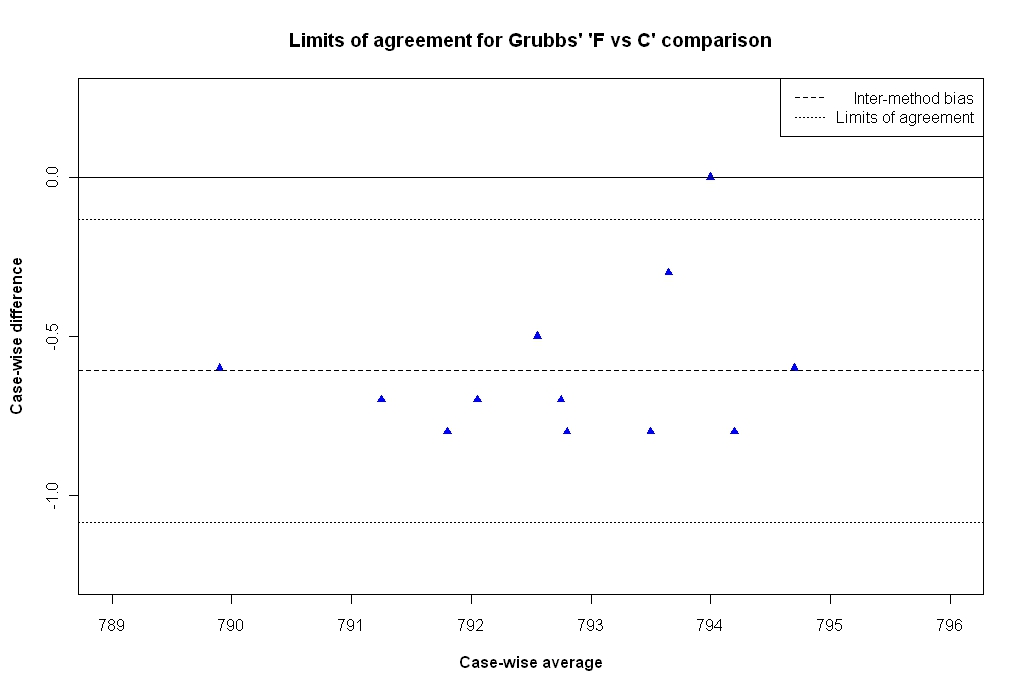
\includegraphics[width=125mm]{GrubbsBAplot-LOA.jpeg}
  \caption{Bland-Altman plot with limits of agreement}\label{GrubbsBAplot-noLOA}
\end{center}
\end{figure}

The limits of agreement methodology assumes a constant level of
bias throughout the range of measurements. As \citet*{BA86} point
out this may not be the case. Bland and Altman advises on how to
calculate of confidence intervals for the inter-method bias and
the limits of agreement. Importantly the authors recommend prior
determination of what would and would constitute acceptable
agreement, and that sample sizes should be predetermined to give
an accurate conclusion.

\begin{quote}
`How far apart measurements can be without causing difficulties
will be a question of judgment. Ideally, it should be defined in
advance to help in the interpretation of the method comparison and
to choose the sample size.'\citep{BA86}
\end{quote}

%\subsubsection{Small Sample Sizes} The limits of agreement are
%estimates derived from the sample studied, and will differ from
%values relevant to the whole population, hence the importance of a
%suitably large sample size. A different sample would give
%different limits of agreement. Student's t-distribution is a well
%known probability distribution used in statistical inference for
%normally distributed populations when the sample size is small
%\citep{student,Fisher3}. Consequently, using 't' quantiles , as
%opposed to standard normal quantiles, may give a more appropriate
%calculation for limits of agreement when the sample size is small.
%For sample size $n=12$ the `t' quantile is 2.2 and the limits of
%agreement are (-0.074,-1.143).
\citet{BA99} note the similarity of limits of agreement to
confidence intervals, but are clear that they are not the same
thing. Interestingly, they describe the limits as ``being like a
reference interval."

Limits of agreement have very similar construction to Shewhart
control limits. The Shewhart chart is a well known graphical
methodology used in statistical process control. Consequently
there is potential for misinterpreting the limits of agreement as
if equivalent to Shewhart control limits. Importantly the
parameters used to determine the limits, the mean and standard
deviation, are not based on any sample used for an analysis, but
on the process's historical values, a key difference with
Bland-Altman limits of agreement.

\citet{BXC2008} regards the limits of agreement as a prediction
interval for the difference between future measurements with the
two methods on a new individual, but states that it does not fit
the formal definition of a prediction interval, since the
definition does not consider the errors in estimation of the
parameters. Prediction intervals, which are often used in
regression analysis, are estimates of an interval in which future
observations will fall, with a certain probability, given what has
already been observed. \citet{BXC2008} offers an alternative
formulation, a $95\%$ prediction interval for the difference
\begin{equation}
\bar{d} \pm t_{(0.975, n-1)}S_{d} \sqrt{1+\frac{1}{n}}
\end{equation}

\noindent where $n$ is the number of subjects. Only for 61 or more
subjects is there a quantile less than 2.

\citet{luiz} describes limits of agreement as tolerance limits. A
tolerance interval for a measured quantity is the interval in
which a specified fraction of the population's values lie, with a
specified level of confidence.

%At least 100 historical
%values must be used to determine the acceptable value (i.e the
%process mean) and the process standard deviation. The principle
%that the mean and variance of a large sample of a homogeneous
%population is a close approximation of the population's mean and
%variance justifies this.

\subsection{Confidence Intervals and Standard Error}
\citet*{BA99} argue that it is possible to estimate confidence
intervals and standard error, if it is assumed that the
differences approximately follow a normal distribution,

 \begin{equation}
  \mbox{Var}(LoA) = (\frac{1}{n}+\frac{1.96^{2}}{2(n-1)})S_{d}^{2}.
 \end{equation}

If $n$ is sufficiently large this can be following approximation
can be used
 \begin{equation}
  \mbox{Var}(LoA) \approx 1.71^{2}\frac{S_{d}^{2}}{n}.
 \end{equation}
Consequently the standard errors of both limits can be
approximated as $1.71 S.E.(\bar{d})$

A $95\%$ confidence interval can be determined, by means of the
\emph{t} distribution with $n-1$ degrees of freedom. \citet*{BA99} comment that such calculations  may be `somewhat
optimistic' on account of the associated assumptions not being
realized.
\addcontentsline{toc}{section}{Bibliography}

\bibliography{transferbib}

\end{document}
